\subsection{Example \#4: single time series analysis with non-harmonic periodic pattern}
\label{S:Example_TRAFFIC}
\subsubsection{Data description}

This case-study is conducted on the traffic loading data collected on the Tamar Bridge \citep{Goulet2017BDLMEmprical,Nguyen2019KRBDLM}. 
The Figure~\ref{fig:DataSummaryTraffic}a shows that data points exist between  September $01$ and October $21$, $2007$. Beyond that date, the timestamps are associated with NaN (i.e. missing data) in order to forecast the predicted traffic load for a period of two weeks (see Figure~\ref{fig:DataSummaryTraffic}c).  
The timestep is $30$\,minutes for all data points (Figure~\ref{fig:DataSummaryTraffic}a).
The time series is stationnary with a level, a periodic pattern with a period of $7$\,days, and autoregressive pattern.
%The traffic loading on weekends is much lighter than those on weekdays. 
%For most of the day, the traffic load presents a high volume between $8$\,am and $4$\,pm, yet it drops out after $20$\,pm at night. 



\begin{figure*}[h]
\centering
\begin{subfigure}{\linewidth}\centering
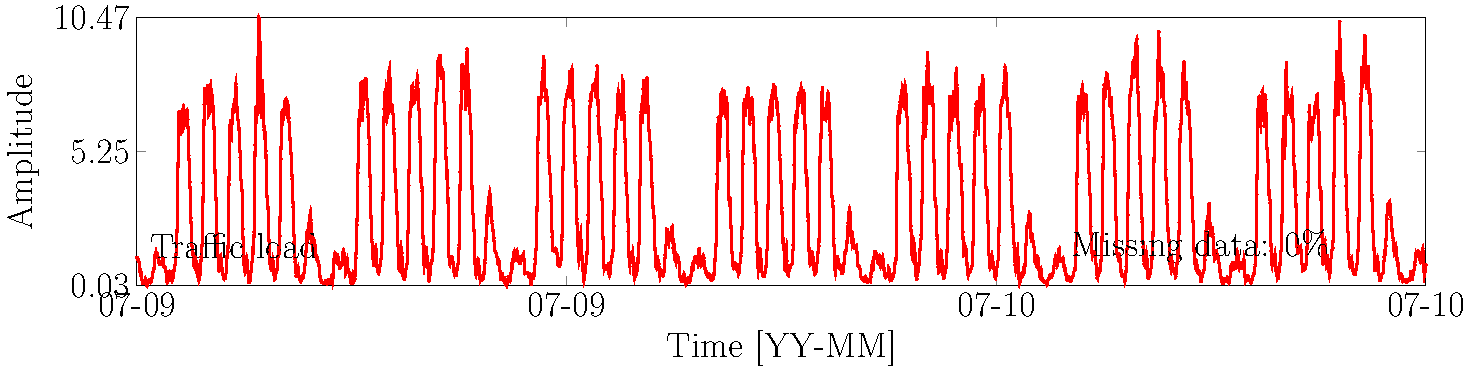
\includegraphics[width=0.9\linewidth]{./docfigs/Example_TRAFFIC/raw/ALL_AMPLITUDES.pdf}
\caption{Amplitude}
\end{subfigure}
\begin{subfigure}{\linewidth}\centering
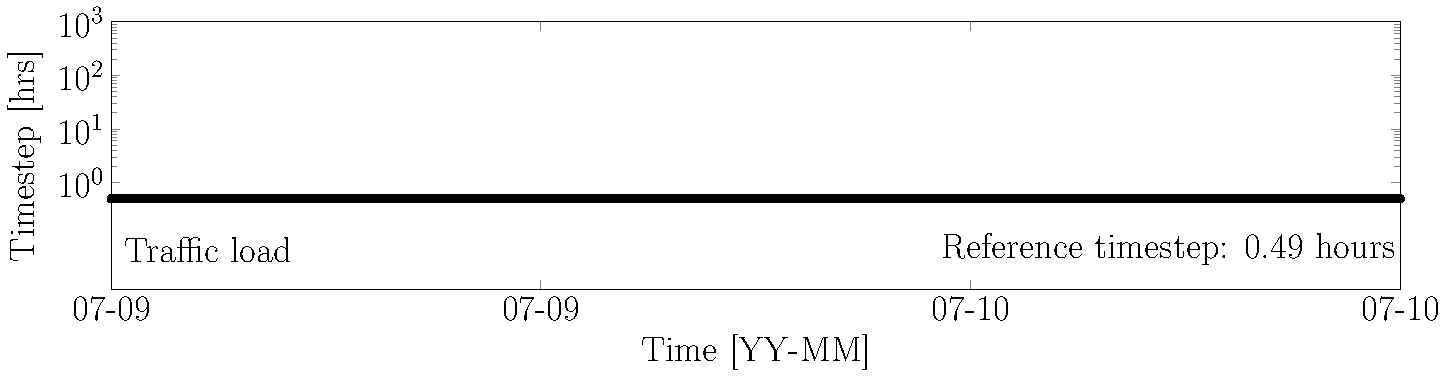
\includegraphics[width=0.9\linewidth]{./docfigs/Example_TRAFFIC/raw/ALL_TIMESTEPS.pdf} 
\caption{Timestep}
\end{subfigure}
\begin{subfigure}{\linewidth}\centering
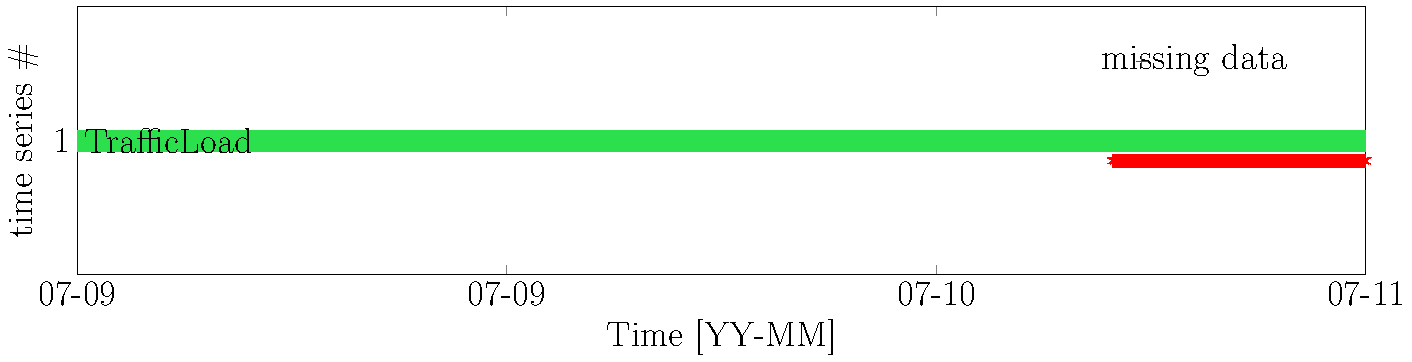
\includegraphics[width=0.9\linewidth]{./docfigs/Example_TRAFFIC/raw/AVAILABILITY.pdf}
\caption{Availability}
\end{subfigure}
\caption{Data used in the example \#4.}
\label{fig:DataSummaryTraffic}
\end{figure*}


\subsubsection{Model description}
\label{SS:ModelConstructionExampleTraffic}

The model includes one model class, and the hidden states variables are 
\begin{gather*}
\begin{array}{rcl}
\mathbf{x} &=& \left[x^{\mathtt{LL}}, x_{0}^{\mathtt{KR}}, x_{1}^{\mathtt{KR}},\cdots,x_{100}^{\mathtt{KR}}, x^{\mathtt{AR}}\right]^{\intercal}.
\end{array}
\end{gather*}
The associated model parameters are
\begin{equation}
\label{EQ:PTL}
\bm\theta = \left[\sigma^{\mathtt{LL}}_{w}, \ell^{\mathtt{KR}}, p^{\mathtt{KR}}, \sigma_{w,0}^{\mathtt{KR}}, \sigma_{w,1}^{\mathtt{KR}}, \phi^{\mathtt{AR}}, \sigma^{\mathtt{AR}}_{w}, \sigma_{v}\right],
\end{equation}
The optimized model parameters values computed using the Newton-Raphson algorithm (see~\ref{SS:THModelParameterEstimation}) with a training period of 14 days are
\begin{gather*}
\bm\theta^{\text{*}}=[0 , 0.052, 7, 2.1\times10^{-5}, 0, 0.81, 0.30, 4.6\times10^{-5}].
\end{gather*}
The optimized initial hidden states mean and covariance values are 
\begin{align*}
%\bm \mu^{*}_{0} & = [	 3.12  ,	0  ,   	-2.28  ,	-1.42  ,	-2.83 ,	-2.66 ,	-3    	,-2.68  \\
%&	-3.04 ,	-2.76 ,	-2.84 ,	-2.46 ,	-2.03 ,	-1.77 ,	-2.29 ,	-1.66  \\
%&	-2.81 ,	-1.12 ,	-3.01 ,	-2.38 ,	-2.94 ,	-2.14 ,	-4.11 ,	-0.562  \\
%&	-5.66 ,	4.08  ,	4.37  ,	2.45  ,	6.1   	2.23  ,	6.65  ,	0.261 ,	2.02  \\
%&	-3.09 ,	-2.05 ,	-1.01 ,	-3.75 ,	-1.3  	-3.71, 	0.13  ,	7.36  ,	1.01  \\
%&	7.83  ,	1.34  ,	6.47  ,	2.51  ,	1.08  ,	-1.13 ,	-3.78 	-0.0821,	-3.46  \\
%&	-2.67 ,	-1.99 ,	-3.81 ,	8.39  ,	0.615 ,	6.58  ,	2.37  	6.78  ,	2.88  \\
%&	1.27  ,	0.435 ,	-4.15 ,	-0.547,	-2.58 ,	-3.7 , 	-0.459	, -5.28  \\
%&	5.88  ,	2.47  ,	6.48  ,	4.43  ,	3.85  ,	6.17  ,	0.338 ,	1.41  \\
%&	-3.44 ,	-1.96 ,	-1.23 ,	-4.17 ,	-0.604,	-4.94 ,	2.38  ,	5.72  \\
%&	3.55  ,	5.32  ,	4.28  ,	4.23  ,	2.63  ,	-0.57 ,	-1.42 ,	-3.68  \\
%&	-0.623,	-4.01 ,	-1.72 ,	-3.56 ,	-1.27 ,	-1.42 ,	0.601 ,	-0.864	 \\
%& -0.961,	-1.48 ,	-0.109]^{\intercal}, \text{and} \\
\bm \mu^{*}_{0} & = [	 3.11  ,	0  ,   	-1.72  ,	-1.87 ,	\dots, -0.126]^{\intercal}, \text{and} \\
\bm\Sigma^{*}_{0} & = \text{diag}[   0.0828,	8.19,  	0.459, 	0.436 , \dots, 0.182 ].
 \end{align*}
The hidden states computed using the estimated model parameters and initial hidden states are presented in Figure~\ref{fig:Example_TrafficOptimizedOptimized}.





\begin{figure*}[h!]
\begin{center}
\begin{subfigure}{\linewidth}\centering
\qquad~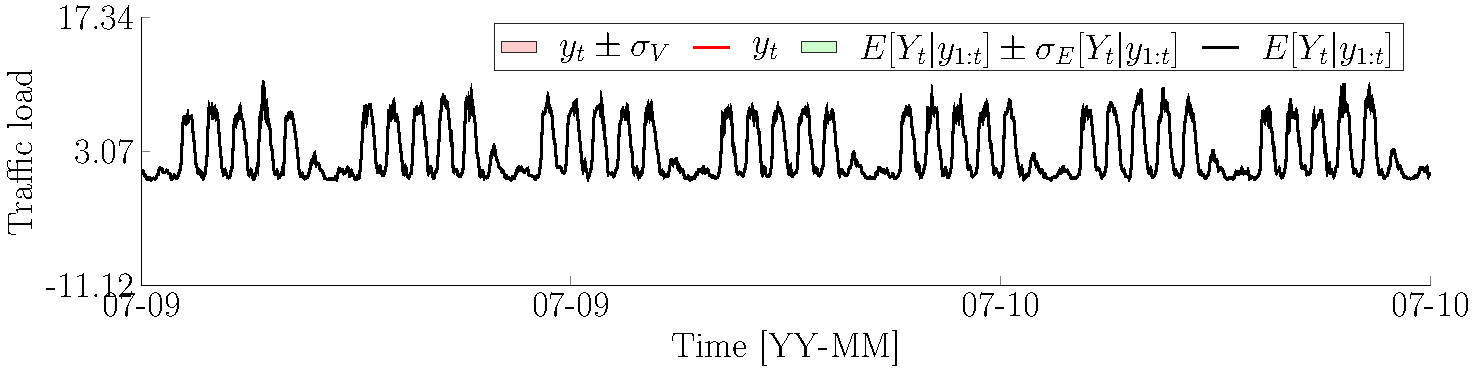
\includegraphics[width=0.83\linewidth]{./docfigs/Example_TRAFFIC/optim_param_optim_initialhiddenstate/TrafficLoad_ObservedPredicted.pdf} 
\caption{Observed and estimated traffic load data}
\end{subfigure}
\begin{subfigure}{\linewidth}\centering
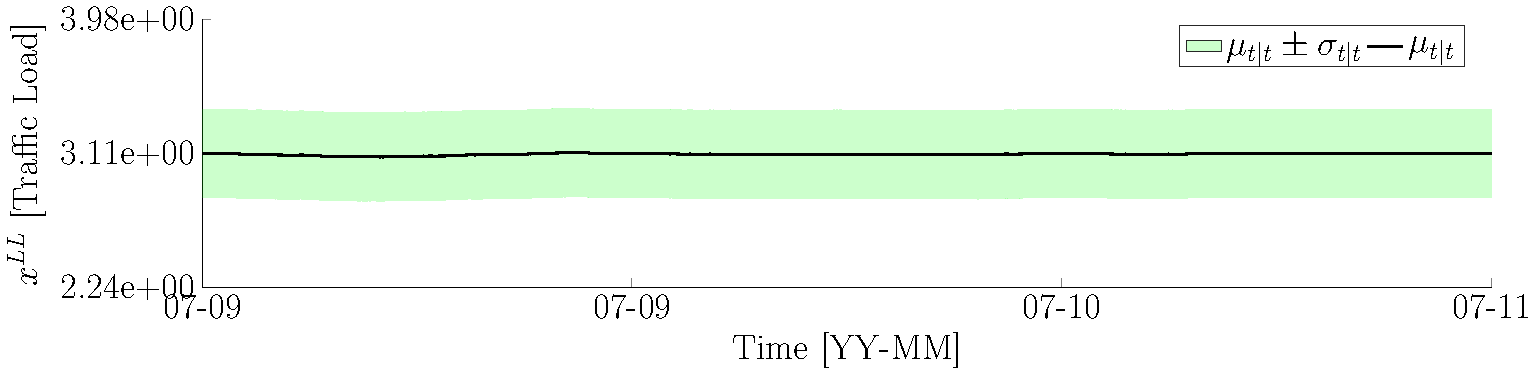
\includegraphics[width=0.9\linewidth]{./docfigs/Example_TRAFFIC/optim_param_optim_initialhiddenstate/TrafficLoad_LL_1.pdf}
\caption{Estimated displacement local level component.}
\end{subfigure}
\begin{subfigure}{\linewidth}\centering
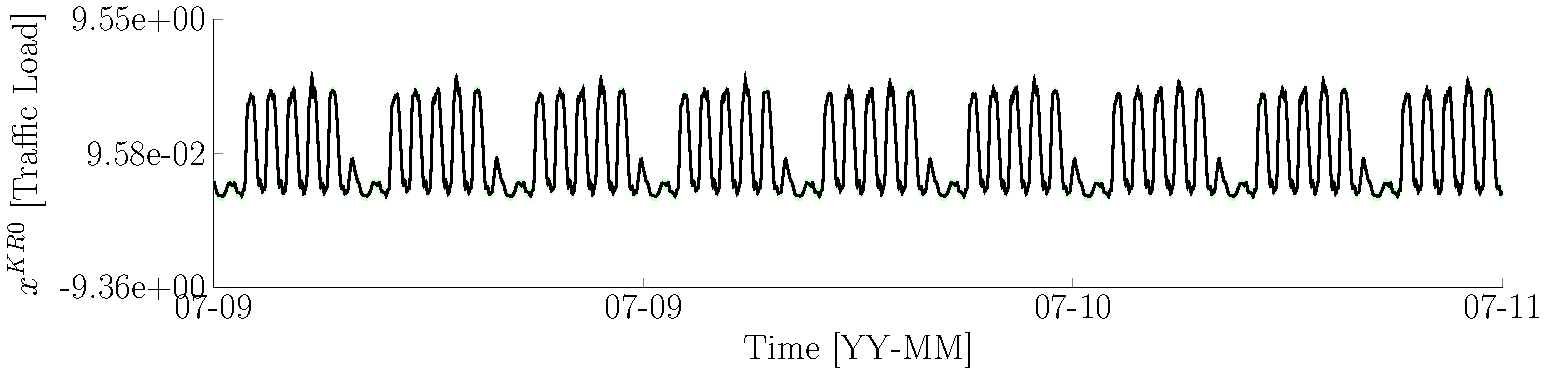
\includegraphics[width=0.9\linewidth]{./docfigs/Example_TRAFFIC/optim_param_optim_initialhiddenstate/TrafficLoad_KR0_2.pdf} 
\caption{Estimated traffic load yearly periodic component (first hidden state)}
\end{subfigure}
\begin{subfigure}{\linewidth}\centering
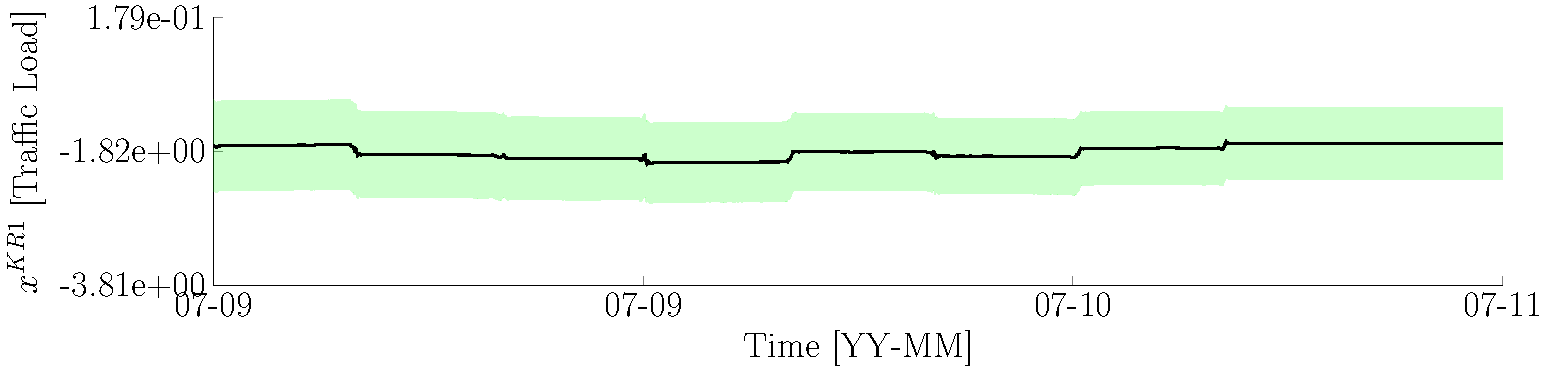
\includegraphics[width=0.9\linewidth]{./docfigs/Example_TRAFFIC/optim_param_optim_initialhiddenstate/TrafficLoad_KR1_3.pdf}
\caption{Estimated traffic load yearly periodic component (second hidden state)}
\end{subfigure}
\begin{subfigure}{\linewidth}\centering
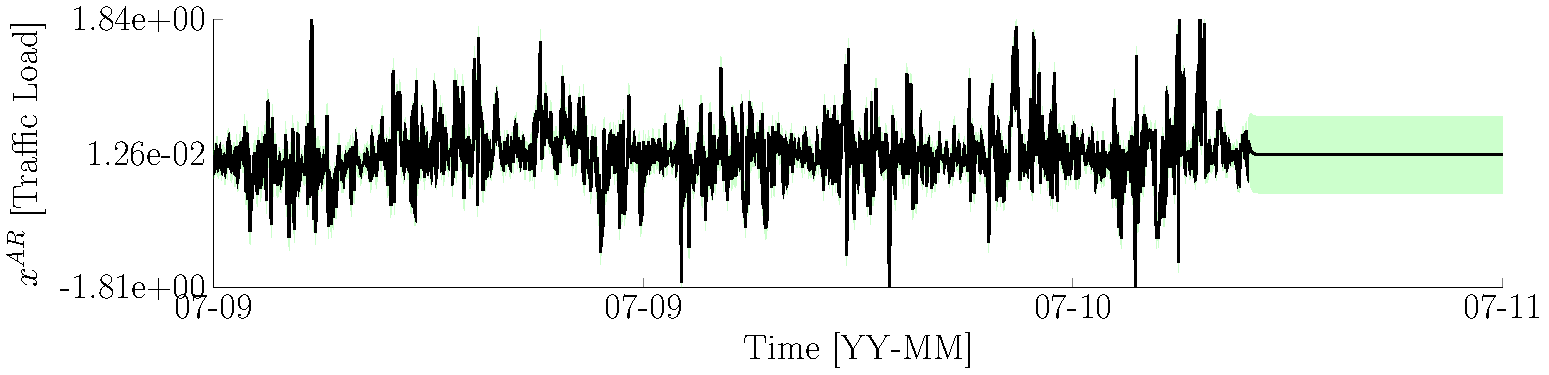
\includegraphics[width=0.9\linewidth]{./docfigs/Example_TRAFFIC/optim_param_optim_initialhiddenstate/TrafficLoad_AR_4.pdf} 
\caption{Estimated traffic load autoregressive component}
\end{subfigure}
\caption{Estimated results using OpenBDLM optimized model parameters and optimized initial hidden states. The hidden states are estimated from the data presented in Figure~\ref{fig:DataSummaryTraffic}a. The solid line and shaded area represent the mean and standard deviation of the estimated hidden states, respectively.}
\label{fig:Example_TrafficOptimizedOptimized}
\end{center}
\end{figure*}



\subsubsection{Run the example from pre-existing configuration file}
\label{SS:LoadConfigFileTraffic}


There is a configuration file CFG\_Example\_TRAFFIC\_optim.m which is located in the ``config\_files'' folder of the OpenBDLM package.
CFG\_Example\_TRAFFIC\_optim.m contains the optimized model parameters and optimized initial hidden states values.
There is also a data file DATA\_Example\_TRAFFIC\_optim.mat that is located in the ``data/mat'' subfolder.
Therefore, it is possible to run the example \#4 by following the steps below while interacting with the \MATLAB{} command line:
\begin{enumerate}
\item Start OpenBDLM. Type \colorbox{light-gray}{\lstinline[basicstyle = \mlttfamily \small, backgroundcolor = \color{light-gray}]!OpenBDLM_main('CFG_Example_TRAFFIC_optim.m');!}.
\item Access hidden states estimation menu. Type \colorbox{light-gray}{\lstinline[basicstyle = \mlttfamily \small, backgroundcolor = \color{light-gray}]!3!}.
\item Run the Kalman filter to estimate the hidden states. Type \colorbox{light-gray}{\lstinline[basicstyle = \mlttfamily \small, backgroundcolor = \color{light-gray}]!1!}.
\item Save and quit. Type \colorbox{light-gray}{\lstinline[basicstyle = \mlttfamily \small, backgroundcolor = \color{light-gray}]!Q!}.
\end{enumerate}


\subsubsection{Run the example from command line interaction}

The analysis of a new dataset usually requires to start from scratch.
This section explains how to run the example \#4 from scratch, that is, how to load the data presented in Figure~\ref{fig:DataSummaryTraffic}, configure the model, estimate the model parameters and estimate the hidden states as presented in Figure~\ref{fig:Example_DISPSIMOptimizedOptimizedExampleTraffic}.
This may be done by following steps below while interacting with the \MATLAB{} command line:
\begin{enumerate}
\item Start OpenBDLM. Type \colorbox{light-gray}{\lstinline[basicstyle = \mlttfamily \small, backgroundcolor = \color{light-gray}]!OpenBDLM_main;!}.
\item Choose the interactive tool. Type \colorbox{light-gray}{\lstinline[basicstyle = \mlttfamily \small, backgroundcolor = \color{light-gray}]!0!}.
\item Enter the project name. Type \colorbox{light-gray}{\lstinline[basicstyle = \mlttfamily \small, backgroundcolor = \color{light-gray}]!Example_TRAFFIC!}. 
\item Disregard generating synthetic data. Type \colorbox{light-gray}{\lstinline[basicstyle = \mlttfamily \small, backgroundcolor = \color{light-gray}]!no!}. 
\item Load new data. Type \colorbox{light-gray}{\lstinline[basicstyle = \mlttfamily \small, backgroundcolor = \color{light-gray}]!0!}.
\item Select from the graphical user interface the data file Example\_TRAFFIC\_TrafficLoad.csv located in the folder ``/data/csv/Example\_TRAFFIC''. The Figure~\ref{fig:DataSummaryTraffic} that represents the raw data should popup on screen.
\item Save and continue without pre-processing. Type \colorbox{light-gray}{\lstinline[basicstyle = \mlttfamily \small, backgroundcolor = \color{light-gray}]!7!}. The Figure~\ref{fig:DataSummaryTraffic} should popup on screen again,.
\item Select the number of model classes. Type \colorbox{light-gray}{\lstinline[basicstyle = \mlttfamily \small, backgroundcolor = \color{light-gray}]!1!}. 
\item Select the model block components. Type \colorbox{light-gray}{\lstinline[basicstyle = \mlttfamily \small, backgroundcolor = \color{light-gray}]![11 51 41]!}.
\item Access model parameters menu. Type \colorbox{light-gray}{\lstinline[basicstyle = \mlttfamily \small, backgroundcolor = \color{light-gray}]!11!}.
\item Modify a model parameter. Type \colorbox{light-gray}{\lstinline[basicstyle = \mlttfamily \small, backgroundcolor = \color{light-gray}]!1!}.
\item Modify the third model parameter (period of the kernel regression component). Type \colorbox{light-gray}{\lstinline[basicstyle = \mlttfamily \small, backgroundcolor = \color{light-gray}]!3!}.
\item Provide new value for  the period. Type \colorbox{light-gray}{\lstinline[basicstyle = \mlttfamily \small, backgroundcolor = \color{light-gray}]!7!}.
\item Provide new bounds for the period. Type \colorbox{light-gray}{\lstinline[basicstyle = \mlttfamily \small, backgroundcolor = \color{light-gray}]![NaN NaN]!}.

\item Access the training period modification menu. Type \colorbox{light-gray}{\lstinline[basicstyle = \mlttfamily \small, backgroundcolor = \color{light-gray}]!13!}. 

\item Modify the training period. Type \colorbox{light-gray}{\lstinline[basicstyle = \mlttfamily \small, backgroundcolor = \color{light-gray}]!1!}. 

\item Choose the starting time (day). Type \colorbox{light-gray}{\lstinline[basicstyle = \mlttfamily \small, backgroundcolor = \color{light-gray}]!1!}. 

\item Choose the end time (day). Type \colorbox{light-gray}{\lstinline[basicstyle = \mlttfamily \small, backgroundcolor = \color{light-gray}]!14!}. 

\item Access model parameter estimation menu. Type \colorbox{light-gray}{\lstinline[basicstyle = \mlttfamily \small, backgroundcolor = \color{light-gray}]!1!}. 
\item Start Newton-Raphson algorithm. Type \colorbox{light-gray}{\lstinline[basicstyle = \mlttfamily \small, backgroundcolor = \color{light-gray}]!1!}. Once the algorithm has converged, the optimized model parameters values should be close to the values presented in Section~\ref{SS:ModelConstructionExampleTraffic}. Note that it is possible to get slightly different value of parameters with the same performance\footnote{Keep in mind that the optimization may take several minutes to several hours. It is possible to abort the analysis here and to load the configuration file called CFG\_Example\_TRAFFIC\_optim.m to load pre-computed values of model parameters, as presented in Section~\ref{SS:LoadConfigFileTraffic}.}.
\item Estimate the initial hidden states values. Type \colorbox{light-gray}{\lstinline[basicstyle = \mlttfamily \small, backgroundcolor = \color{light-gray}]!2!}.
\item Access hidden states estimation menu. Type \colorbox{light-gray}{\lstinline[basicstyle = \mlttfamily \small, backgroundcolor = \color{light-gray}]!3!}. 
\item Estimate the filtered hidden states. Type \colorbox{light-gray}{\lstinline[basicstyle = \mlttfamily \small, backgroundcolor = \color{light-gray}]!1!}. The estimation should be similar to the results presented in Figure~\ref{fig:Example_DISPSIMOptimizedOptimizedExample1}.
\item Access export menu. Type \colorbox{light-gray}{\lstinline[basicstyle = \mlttfamily \small, backgroundcolor = \color{light-gray}]!17!}. 
\item Export the current project in a configuration file. Type \colorbox{light-gray}{\lstinline[basicstyle = \mlttfamily \small, backgroundcolor = \color{light-gray}]!1!}.
\item Save and quit OpenBDLM. Type \colorbox{light-gray}{\lstinline[basicstyle = \mlttfamily \small, backgroundcolor = \color{light-gray}]!Q!}.
\end{enumerate}


